\newpage % Rozdziały zaczynamy od nowej strony.
\section{Main objective}

The main objective of this thesis is to demonstrate how knowledge graphs can be
used in the medical domain in combination with experimental data, i.e.,
real-world patient data. The thesis addresses two tasks:
\begin{itemize}[label=\textendash]
    \item \textbf{Task A: Link prediction}, which reconstructs and updates the
    knowledge graph on the basis of real-world patient data;
    \item \textbf{Task B: Patient risk prediction} (a node-classification task),
    which predicts clinical outcomes using the knowledge graph
    and real-world patient data.
\end{itemize}

The two tasks are complementary and could
form a closed-loop approach to patient-centred care in a real-world medical setting. 
Link prediction focused more on sharing medical knowledge between different stakeholders 
(hospitals, clinicians, patients), while risk prediction focuses on the 
individual patient outcomes.
 As shown in Figure \ref{fig:loop}, these two tasks could operate as 
 an iterative process for improving patient care.

\begin{figure}[h]
    \centering
    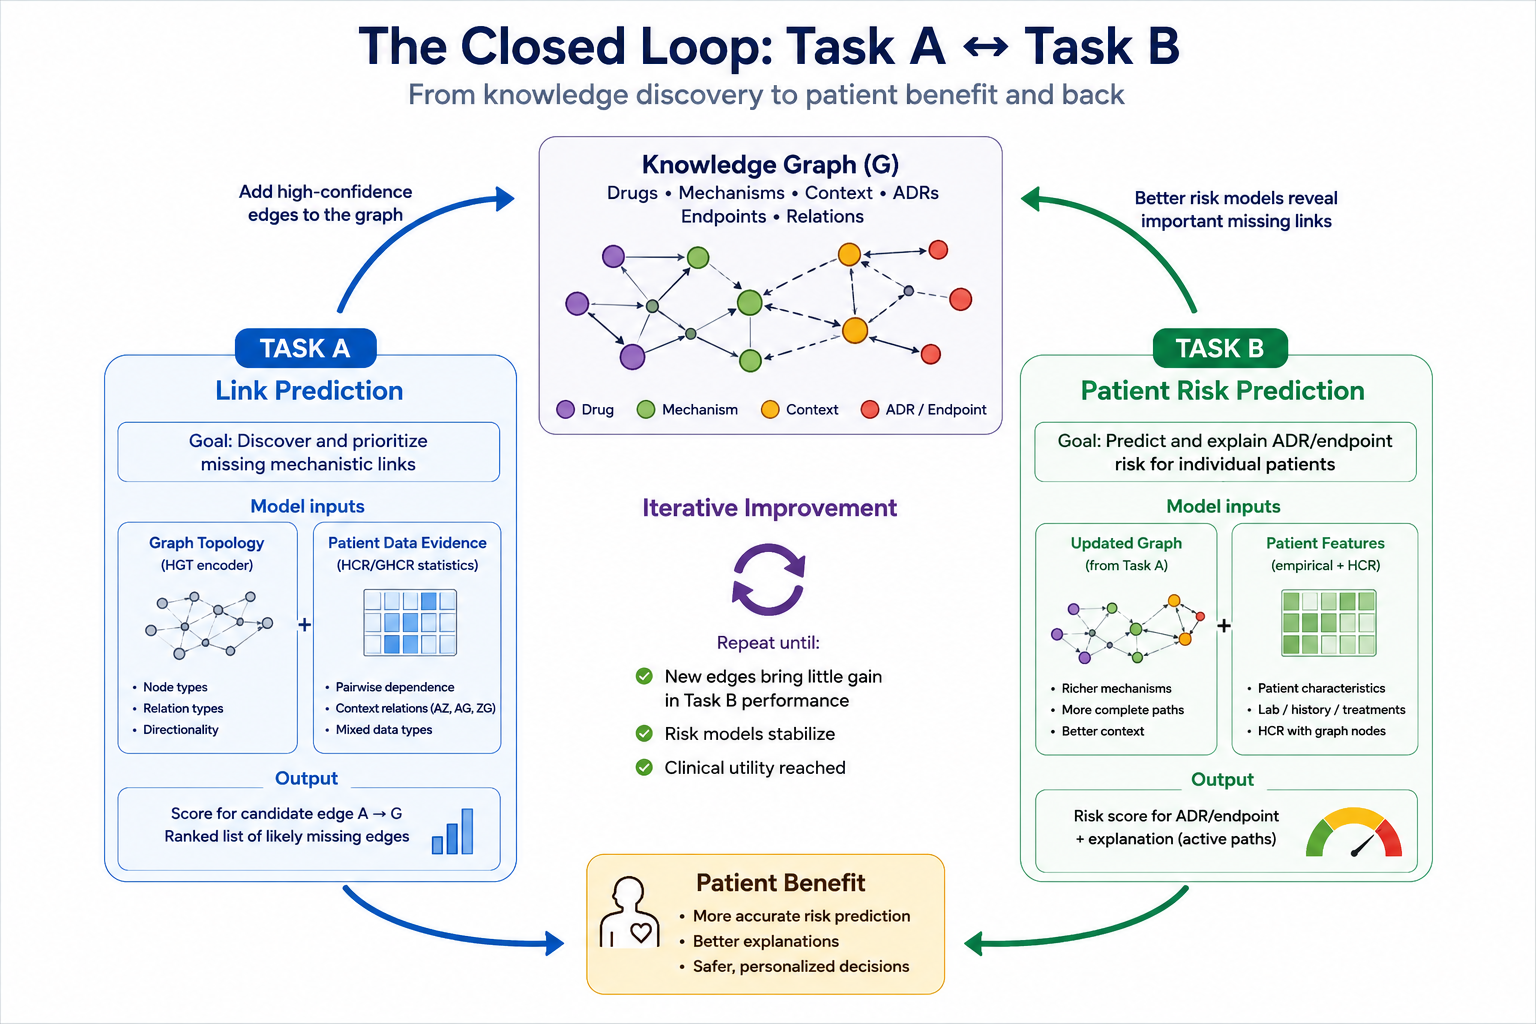
\includegraphics[width=\textwidth, height=0.45\textheight]{rysunki/TASK A i B - loop.png}
    \caption{Overview of the two tasks addressed in this thesis.}
    \label{fig:loop}
\end{figure}
In addition to this domain-oriented objective, the thesis investigates
heterogeneous GNNs enhanced with an additional layer for calculating
dependencies between nodes, namely Hierarchical Correlation Reconstruction
(HCR). This approach examines whether GNNs can be improved by incorporating
statistical dependencies without requiring computationally costly extensions
to the model architecture.